%
\documentclass{article}

% Encoding of the file
\usepackage[utf8]{inputenc}

% Font: computer modern bright
%\usepackage{cmbright}

% math packages
\usepackage{amsmath,amssymb,MnSymbol}
\usepackage[dvips]{graphicx}
\usepackage{psfrag,comment}
%\usepackage[T1]{fontenc}
%\usepackage{amsfonts}

\title{Sound Field Synthesis}

%\graphicspath{{figs/}}

% Include some macros from external file
% latex macros for signals and transformations
% S.Spors, 11.11.05


\renewcommand{\vec}[1]{\ensuremath{ \mathbf{#1} }}

%=============== some macros =================================================
\newcommand{\eg}[0]{e.\,g.}
\newcommand{\qc}[0]{\;,}
\newcommand{\qp}[0]{\;.}
\newcommand{\threeD}[0]{\text{3D}}
\newcommand{\twoD}[0]{\text{2D}}
\renewcommand{\comment}[1]{{\color{magenta}{#1}}}


%=============== References ==================================================
\newcommand{\FigRef}[1]{Fig.~\ref{#1}}
\newcommand{\TblRef}[1]{Table~\ref{#1}}
\newcommand{\SecRef}[1]{Section~\ref{#1}}
\newcommand{\AppRef}[1]{Appendix~\ref{#1}}
\newcommand{\PRef}[1]{Page~\pageref{#1}}
\newcommand{\EqRef}[1]{Eq.~(\ref{#1})}

\newcommand{\ul}[1]{\underline{#1}}


%=============== Funktionen =========================================
\newcommand{\omegac}{\frac{\omega}{c}}

% Variablen, Vektoren, . . .
\newcommand{\x}{\ensuremath{ \vec{x} }}
\newcommand{\n}{\ensuremath{ \vec{n} }}
% x-x_0 (vector)
\newcommand{\xx}{\ensuremath{ \vec{x}-\vec{x}_0 }}
% k (vector) 
% NOTE: the \k command is for the ogonek accent, which we very probably will 
% not need, therefore I overwrite it
\renewcommand{\k}{\ensuremath{ \vec{k} }}

%=============== Matrizen & Vektoren =========================================
\newcommand{\Vek}[1]{\ensuremath{ \mathbf{#1} }}
\newcommand{\Mat}[1]{\ensuremath{ \mathbf{#1} }}
\newcommand{\FSc}[1]{\ensuremath{ \underline{#1} }}
\newcommand{\FVek}[1]{\ensuremath{ \underline{\mathbf{#1}} }}
\newcommand{\FMat}[1]{\ensuremath{ \underline{\mathbf{#1}} }}
\newcommand{\FFSc}[1]{\ensuremath{\underline{\underline{#1}}}}
\newcommand{\FFVek}[1]{\ensuremath{\underline{\underline{\mathbf{#1}}}}}
\newcommand{\FFMat}[1]{\ensuremath{\underline{\underline{\mathbf{#1}}}}}
%\newcommand{\FFSc}[1]{\ensuremath{\uuline{#1}}}
%\newcommand{\FFVek}[1]{\ensuremath{\uuline{\mathbf{#1}}}}
%\newcommand{\FFMat}[1]{\ensuremath{\uuline{\mathbf{#1}}}}
\newcommand{\TP}[1]{\ensuremath{ #1^T }}
\newcommand{\HE}[1]{\ensuremath{ #1^H }}
\newcommand{\norm}[1]{\ensuremath{ \left\| #1 \right\|}}
\newcommand{\ABS}[1]{\ensuremath{ \left| #1 \right|}}
\newcommand{\dotprod}[2]{{\ensuremath{\langle#1,#2\rangle}}}
\newcommand{\diag}[1]{\ensuremath{\text{diag} \{ #1 \} }}
\newcommand{\Bdiag}[1]{\ensuremath{\text{Bdiag} \{ #1 \} }}
\newcommand{\mvec}[1]{\ensuremath{\text{vec} \{ #1 \} }}
\newcommand{\rank}[1]{\ensuremath{\text{rk} \{ #1 \} }}
\newcommand{\tr}[1]{\ensuremath{\text{tr} \{ #1 \} }}

\newcommand{\pos}[1]{\ensuremath{(#1)}}


\newcommand{\defeq}{\mathrel{\!\mathop:}=}

%%%%%%%%%%%%%%%%%%%%%%%%%%%%%%%%%%%%%%%%%%%%%%%%%%%%%%%%%%%%%%%%%%%%%%%%%%%%%%%%
\begin{document}

\maketitle

\section{Wave equation}

Hier kurz auf die Lösungen der Wellengleichung eingehen, Fourier-Trafo
definieren und die entsprechenden Lösungen und Greenschen Funktionen einführen.

%%%%%%%%%%%%%%%%%%%%%%%%%%%%%%%%%%%%%%%%%%%%%%%%%%%%%%%%%%%%%%%%%%%%%%%%%%%%%%%%
\section{Single Layer Potential}
\label{sec:singlelayerpotential}

The acoustic pressure $P(\x,\omega)$ synthesized by a weighted distribution
of monopole sources (\emph{single layer potential}) located on the
surface $\partial V$ of an open area $V \subset \mathbb{R}^3$ is given as
\begin{equation}
    P(\x,\omega) = \oint_{\partial V} \!\! G(\x|\x_0,\omega) D(\x_0,\omega) \, 
    dA(\x_0) \qc
    \label{eq:singlelayer}
\end{equation}
where $G(\x|\x_0,\omega)$ denotes the sound field of a monopole
source located at $\x_0 \in \partial V$ and $D(\x_0,\omega)$ its weight which usually
is referred to as driving signal. The geometry of the problem is illustrated in
Figure~\ref{fig:KHint}.
\begin{figure}
    \psfrag{source}[][][1]{\shortstack{virtual\\source}}
    \psfrag{S}[][][1]{$S(\x,\omega)$}
    \psfrag{P}[l][][1]{$P(\x,\omega)$}
    \psfrag{x}[][][1]{$\x$}
    \psfrag{x_0}[][][1]{$\x_0$}
    \psfrag{n}[][][1]{$\n$}
    \psfrag{V}[][][1]{$V$}
    \psfrag{dV}[][][1]{$\partial V$}
    \psfrag{0}[][][1]{$0$}
    \centerline{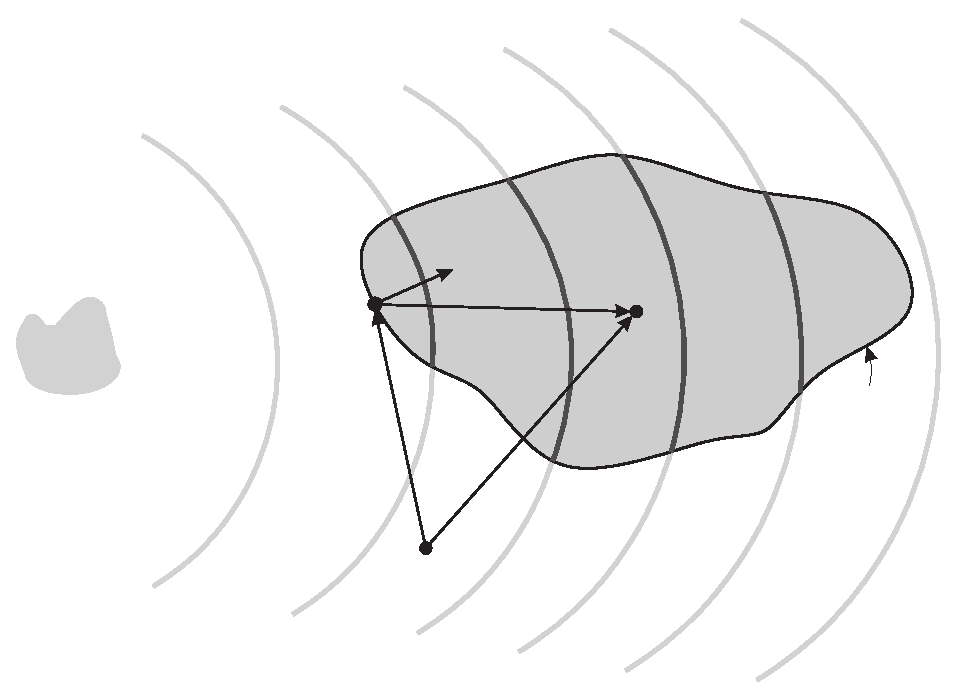
\includegraphics[scale=0.5]{KHint}}
    \caption{Illustration of the geometry used to discuss the physical foundations of sound field synthesis
    and the single layer potential~\eqref{eq:singlelayer}.}
    \label{fig:KHint}
\end{figure}
In SFS the monopole sources are referred to as secondary sources. Under free-field conditions,
their sound field $G(\x|\x_0,\omega)$ is given by the three dimensional Greens
function~\cite{Williams1999}. The task is to find the appropriate driving
signals $D(\x_0,\omega)$ for the synthesis of a virtual source $P(\x,\omega) = S(\x,\omega)$
within $V$. It has been shown~\cite{Fazi2009} that the integral equation~\eqref{eq:singlelayer}
can be solved in principle.

%%%%%%%%%%%%%%%%%%%%%%%%%%%%%%%%%%%%%%%%%%%%%%%%%%%%%%%%%%%%%%%%%%%%%%%%%%%%%%%%
\subsection{Explicit Solution (HOA, SDM)}%
\label{sec:explicitsolution}
%
One approach is to explicitly solve the integral equation~\eqref{eq:singlelayer} with
respect to the driving signals $D(\x_0,\omega)$. According to operator
theory~\cite{Giroire1982,Fazi2008,Spors2008b},
this integral equation is a (compact) Fredholm operator of zero index. Its solution is hence given
by expanding the kernel, the driving signal and the virtual sound field into a series
of orthogonal basis functions. Suitable basis functions can be found for arbitrary simply
connected domains $V$ with a smooth boundary. However, analytic basis functions are in practice
only available for regular geometries like spheres, circles, planes and lines. For spheres,
and circles the resulting family of solutions is known as (Near-Field Compensated) Higher-Order
Ambisonics~\cite{Daniel2001,Poletti2005,Fazi2008,Ahrens2008a}. For planes, and lines as
Spectral Division Method (SDM)~\cite{Ahrens2010a,Ahrens2008}.
The driving functions for these two approaches are given in section
\ref{sec:hoa25d} and section \ref{sec:sdm25d}, respectively.

%%%%%%%%%%%%%%%%%%%%%%%%%%%%%%%%%%%%%%%%%%%%%%%%%%%%%%%%%%%%%%%%%%%%%%%%%%%%%%%%
\subsection{Implicit Solution (WFS)}
\label{sec:implicitsolution}
%
The single layer potential~\eqref{eq:singlelayer} satisfies the homogeneous
Helmholtz equation both in the interior and exterior regions $V$ and
$\bar{V} \defeq \mathbb{R}^3 \setminus (V \cup \partial V)$.
If $D(\x,\omega)$ is continuous, its pressure value $P(\x,\omega)$ is continuous when approaching
the surface $\partial V$ from the inside and outside.
Due to the presence of the secondary sources at the
surface $\partial V$, the gradient of $P(\x,\omega)$ is discontinuous when approaching the surface
$\partial V$. As a consequence, $\partial V$ can be
interpreted as the boundary of scattering object with Dirichlet boundary
conditions~\cite{Fazi2009}, hence as a sound-soft object.
Considering this {\em equivalent scattering problem}, the driving signal is given
as~\cite{Williams1999,Fazi2009}
\begin{equation}
    D(\x_0,\omega) = \frac{\partial}{\partial \n} S_\text{i}(\x_0,\omega) -
    \frac{\partial}{\partial \n} S_\text{s}(\x_0,\omega)\qc
\end{equation}
where $S_\text{i}(\x,\omega), \; \x\in V$ denotes the sound field within $V$,
$S_\text{s}(\x,\omega), \; \x\in \bar{V}$ the scattered field, and
$\frac{\partial}{\partial \n}\!\defeq\!\langle\nabla \cdot,\n\rangle$ the
directional gradient evaluated at the position $\x$. Acoustic scattering problems can
be solved analytically for simple geometries of the surface $\partial V$, like spheres
or planes~\cite{Bowman87:Book}.

Of special interest is the solution for an infinite planar
boundary $\partial V$.
For this specialized geometry and Dirichlet boundary conditions, the driving function is
given as~\cite{Williams1999}
\begin{equation}
    D(\x_0,\omega) = 2 \frac{\partial}{\partial \n} S(\x_0,\omega)\qc
    \label{eq:dwfs}
\end{equation}
since the scattered pressure is the reverse of the interior pressure.
The integral equation resulting from introducing~\eqref{eq:dwfs} into~\eqref{eq:singlelayer}
for a planar boundary $\partial V$ is known as {\em Rayleigh's first integral
equation}~\cite{Williams1999}.

An approximate solution of the solution for planar boundaries can be found by applying the
\emph{Kirchoff approximation}~\cite{Colton83:Book}. Here it is assumed that a bend surface can be
approximated by a set of small planar surfaces for which~\eqref{eq:dwfs} holds locally.
In general this will be the case if the wave length is much smaller than the
dimensions of the boundary,
hence for high frequencies. In addition only that part of the surface is active
which is illuminated from the incident field of the virtual source. That implies also that
we can use only convex surfaces to avoid contributions from outside of the listening
area $V$ to reenter. The outlined principle can be formulated by introducing a window function
$w(\x_0)$ into~\eqref{eq:dwfs}
\begin{equation}
S(\x,\omega) \approx \oint_{\partial V}  G_0(\x|\x_0,\omega) \, \underbrace{2 w(\x_0)
\frac{\partial}{\partial \n} S(\x_0,\omega)}_{D(\x_0,\omega)} \; d A(\x_0) \qc
\label{eq:WFSgeneral}
\end{equation}
where $w(\x_0)$ describes a window function for the selection of the secondary sources
accordingly to the criterion given above. Equation~\eqref{eq:WFSgeneral} constitutes
an approximation of the Rayleigh integral which forms the basis for sound
reproduction methods known as Wave Field Synthesis
(WFS)~\cite{Berkhout1988,Verheijen1997,Start1997,Spors2008}. The dricing functions
for WFS will be presented in sections \ref{sec:wfs25d,sec:wfs2d}.

%%%%%%%%%%%%%%%%%%%%%%%%%%%%%%%%%%%%%%%%%%%%%%%%%%%%%%%%%%%%%%%%%%%%%%%%%%%%%%%%
\subsection{Model-based Rendering}
\label{sec:modelbasedrendering}
%
The pressure field of the desired virtual source $S(\x,\omega)$ has to be known
in order to derive the driving signal for the secondary source distribution.
It can either be measured, i.e.~recorded, or modeled. While the former is known as
{\em data-based rendering}, the latter is known as {\em model-based rendering}.
Often applied models in model-based rendering are plane waves, point sources or
sources with a prescribed complex directivity.
In the following the models used within the SFS-Toolbox are presented.

\subsubsection{Plane Wave}
\label{sec:planewave}
The source model for a plane wave is given by~\cite{Williams1999}, S.21, eq. 2.24:
%
\begin{equation} 
    S(\x,\omega) = A(\omega) e^{i\omegac \n \x}
    \qc
\end{equation}
%
where $A(\omega)$ denotes the frequency spectrum of the plane
wave and $\n$ points into the direction of the plane wave.

\subsubsection{Point Source}
\label{sec:pointsource}
The source model for a point source is given by the three dimensional Greens
function~\cite{Williams1999}, S. 198, eq. 6.73:
%
\begin{equation}
    S(\x,\omega) = A(\omega) \frac{1}{4\pi}
    \frac{e^{i\omegac|\x-\x_\text{s}|}}{|\x-\x_\text{s}|}
    \qp
\end{equation}

\subsubsection{Line Source}
\label{sec:linesource}

\subsubsection{Focused Source}
\label{sec:focsudedsource}

%
% ================================================================================
\subsection{2.5-dimensional Reproduction}%
\label{sec:25d_reproduction}%
%
Loudspeaker arrays are often arranged within a two-dimensional space, for example as a
linear or circular array. From a theoretical point of view, the characteristics of the
secondary sources in such setups should conform to the two-dimensional free-field Green's
function. Its sound field can be interpreted as the field produced by a line
source~\cite{Williams1999}. Loudspeakers exhibiting the
properties of acoustic line sources are not practical. Using point
sources as secondary sources for the reproduction in a plane results
in a dimensionality mismatch, therefore such methods are often
termed as {\em 2.5-dimensional reproduction}.

Using a far-field approximation ($\omegac|\xx| \gg 1$) the following
relationship between the two dimensional line source and the three dimensional
point source can be derived~\cite{Williams1999}.
\begin{equation}
    \underbrace{
        \frac{i}{4} \hankelone{0}\left(\omegac |\xx|\right)
    }_{G_\twoD(\xx,\omega)}
    \approx 
    \sqrt{2\pi \frac{ic}{\omega} |\xx|}\;\;
    \underbrace{
        \frac{1}{4 \pi} \frac{e^{i\omegac|\xx|}}{|\xx|}
    }_{G_\threeD(\xx,\omega)} \qp
\label{eq:2D_Green_approx}
\end{equation}
This results in the so called 2.5D driving function, which is given with
\EqRef{eq:2D_Green_approx} as
\begin{equation}
    D_\twohalfD(\x_0,\omega) = \\ 
        \sqrt{ \frac{ic}{\omega} } \;
        \underbrace{\sqrt{2\pi|\x_\text{ref}-\x_0|}}_{g_0} \;
        D_\twoD(\x_0,\omega) \qc 
\label{eq:D_25D}
\end{equation}
where $g_0$ is a geometry dependent constant [Zitat]. It is obvious, that
$g_0$ can be chosen in a way, that the amplitude is correct at a line at
$y_\text{ref}$ parallel to the loudspeaker array.

It is well known from
WFS and HOA, that 2.5-dimensional reproduction techniques suffer
from artifacts~\cite{Verheijen:PhD,Ahrens08:Acta}. Most prominent
are amplitude deviations. Similar artifacts will also be present in other sound reproduction
approaches which aim at correct reproduction in a plane using secondary point
sources.


%%%%%%%%%%%%%%%%%%%%%%%%%%%%%%%%%%%%%%%%%%%%%%%%%%%%%%%%%%%%%%%%%%%%%%%%%%%%%%%%
\section{Driving functions}
\label{sec:drivingfunctions}

\subsubsection{2.5D HOA}
\label{sec:hoa25d}
For circular/spherical secondary source distributions, the required
basis functions are given by spherical harmonics~\cite{Ahrens08:Acta,Wu08:ICASSP,Fazi:PhD}.
Expressing the virtual source $S(\Vek{x},\omega)$, the secondary sources
$G_0(\Vek{x}-\Vek{x}_0,\omega)$ and the driving function
$D(\Vek{x}_0,\omega)$ by spherical harmonics series expansions,
exploiting the orthogonality of the basis functions and performing a
comparison of coefficients turns~\eqref{eq:singlelayer} into a scalar
multiplication of the spherical harmonics expansion coefficients.
Data-based rendering is the traditional rendering technique used in the context of Ambisonics.
The expansion coefficients are here extracted from microphone array recordings,
transmitted and then used for derivation of the driving signal. This
procedure is often referred to as {\em en- and decoding}.
For model-based rendering analytic expressions for the expansion
coefficients are required for the secondary and virtual sources. These can be
derived straightforward for point sources and plane waves~\cite{Ahrens08:Acta}.
As an example, we will illustrate the procedure for the reproduction of a
plane wave using a circular distribution of secondary sources.\\

\subsection{2.5D SDM}
\label{sec:sdm25d}

\subsubsection{Plane Waves}
The source model for a point source is given by [Williams]:
\begin{equation} 
    S(\x,\omega) = 
    \hat{S}_\text{s}(\omega)
    e^{i\omegac \vec{n}_k \x}
    \qc
\end{equation}
where $\hat{S}_\text{s}(\omega)$ denotes the frequency spectrum of the plane
wave and $\vec{n}_k$ the direction of $\vec{k}$, which is the direction of the
plane wave.

Using \EqRef{eq:D} and \EqRef{eq:D_25D} this leads to a driving function of:
\begin{equation}
    D_\twohalfD(\x_0,\omega) = \hat{S}_\text{s}(\omega)
    2 g_0 n_{ky_0} \sqrt{\frac{\omega}{ic}}
    e^{i\omegac \vec{n}_k \x_0}
    \qp
    \label{Dpw}
\end{equation}


%%%%%%%%%%%%%%%%%%%%%%%%%%%%%%%%%%%%%%%%%%%%%%%%%%%%%%%%%%%%%%%%%%%%%%%%%%%%%%%%
\subsubsection{Point Sources}
The source model for a point source is given by [Williams]:
\begin{equation} 
    S(\x,\omega) = 
    \hat{S}_\text{s}(\omega)
    \frac{1}{4\pi} \frac{e^{i\omegac|\x-\x_\text{s}|}}{|\x-\x_\text{s}|}
    \qc 
\end{equation}
where $\hat{S}_\text{s}(\omega)$ denotes the frequency spectrum of the point
sink and $\x_\text{s} = \binom{x_\text{s}}{y_\text{s}}$ the position of the
point source with $y_\text{s} < 0$.
Using \EqRef{eq:D} and \EqRef{eq:D_25D} this leads to a driving function of:
\begin{equation}
    D_\twohalfD(\x_0,\omega) = \hat{S}_\text{s}(\omega)
    \frac{g_0}{2\pi}
    \left( \sqrt{\frac{\omega}{ic}} - \sqrt{\frac{ic}{\omega}} 
    \frac{1}{|\x_0-\x_\text{s}|} \right)
    \frac{y_0-y_\text{s}}{|\x_0-\x_\text{s}|^{2}} 
    e^{i\omegac|\x_0-\x_\text{s}|}
    \qp
    \label{eq:Dps}
\end{equation}


%%%%%%%%%%%%%%%%%%%%%%%%%%%%%%%%%%%%%%%%%%%%%%%%%%%%%%%%%%%%%%%%%%%%%%%%%%%%%%%%
\subsubsection{Focused Sources}

For the synthesis of a focused source, a synthesized wave field is desired which
converges towards a focus point and diverges after passing the focus point.
This is given by a point sink [Williams]:
\begin{equation} 
    S(\x,\omega) = 
    \hat{S}_\text{s}(\omega)
    \frac{1}{4\pi} \frac{e^{-i\omegac|\x-\x_\text{s}|}}{|\x-\x_\text{s}|}
    \qc 
\end{equation}
where $\hat{S}_\text{s}(\omega)$ denotes the frequency spectrum of the point
sink and $\x_\text{s} = \binom{x_\text{s}}{y_\text{s}}$ the position of the
focused source with $y_\text{s} > 0$.
Using \EqRef{eq:D} and \EqRef{eq:D_25D} this leads to a driving function of:
\begin{equation}
    D_\twohalfD(\x_0,\omega) = -\hat{S}_\text{s}(\omega)
    \frac{g_0}{2\pi}
    \left( \sqrt{\frac{\omega}{ic}} + \sqrt{\frac{ic}{\omega}} 
    \frac{1}{|\x_0-\x_\text{s}|} \right)
    \frac{y_0-y_\text{s}}{|\x_0-\x_\text{s}|^{2}} 
    e^{-i\omegac|\x_0-\x_\text{s}|}
    \qp
    \label{eq:Dfs}
\end{equation}
In \FigRef{fig:WFS} the wave field $P(\vec{x},\omega)$ for
a monochromatic focused
source located at $\vec{x}_\text{s} = \binom{0}{1}$ is simulated. The secondary
source distribution is located at the $x$-axis. The wave field converges for
$0<y<1$\,m towards the position of the focused source and diverges for $y>1$\,m
which defines the listening area for the given focused source position.

If the driving function \EqRef{eq:Dfs}
is transferred into the temporal domain,
it is given as
\begin{equation}
    d_{\text{2.5D}}(\x_0,t) = -s(t) * h(t) *
    \frac{g_0}{2\pi}
    \frac{y_0 - y_\text{s}}{|\x_0-\x_\text{s}|^{2}}
    \;\delta\left(t + \frac{|\x_0-\x_\text{s}|}{c}\right)
    \qc
\label{eq:d}
\end{equation}
where $c$ is the speed of sound and
$h(t)$ denotes the inverse Fourier transformation
\begin{equation} 
    h(t) =
    \IFT{\biggl\{ \sqrt{\frac{\omega}{ic}} + \sqrt{\frac{ic}{\omega}}
    \frac{1}{|\x_0-\x_\text{s}} \biggr\}} 
    \qp
    \label{eq:h}
\end{equation}


\subsection{2.5D WFS}
\label{sec:wfs25d}

\subsubsection{Plane Waves}
The source model for a plane wave is given by [Williams, S.21, eq. 2.24]:
\begin{equation} 
    S(\x,\omega) = 
    \hat{S}_\text{s}(\omega)
    e^{i\omegac \vec{n}_k \x}
    \qc
\end{equation}
where $\hat{S}_\text{s}(\omega)$ denotes the frequency spectrum of the plane
wave and $\vec{n}_k$ the direction of $\vec{k}$, which is the direction of the
plane wave.
Using \EqRef{eq:D} and \EqRef{eq:D_25D} this leads to a driving function of
\begin{equation}
    D_\twohalfD(\x_0,\omega) = \hat{S}_\text{s}(\omega)
    2 g_0 n_{ky_0} \sqrt{\frac{\omega}{ic}}
    e^{i\omegac \vec{n}_k \x_0}
    \qp
    \label{Dpw}
\end{equation}

If we use the Fourier transfomation we will get as the driving function for the
time domain
\begin{equation}
    d_\twohalfD(\x_0,t) = s(t) * h(t) * 2 g_0 n_{ky_0} \delta(t +
    \frac{\vec{n}_k \x_0}{c})
    \qc
    \label{dpw}
\end{equation}
where $h(t) = \IFT{\left\{ \sqrt{\frac{\omega}{ic}} \right\}}$.
%%%%%%%%%%%%%%%%%%%%%%%%%%%%%%%%%%%%%%%%%%%%%%%%%%%%%%%%%%%%%%%%%%%%%%%%%%%%%%%%
\subsubsection{Point Sources}
The source model for a point source is given by [Williams]:
\begin{equation} 
    S(\x,\omega) = 
    \hat{S}_\text{s}(\omega)
    \frac{1}{4\pi} \frac{e^{i\omegac|\x-\x_\text{s}|}}{|\x-\x_\text{s}|}
    \qc 
\end{equation}
where $\hat{S}_\text{s}(\omega)$ denotes the frequency spectrum of the point
sink and $\x_\text{s} = \binom{x_\text{s}}{y_\text{s}}$ the position of the
point source with $y_\text{s} < 0$.
Using \EqRef{eq:D} and \EqRef{eq:D_25D} this leads to a driving function of:
\begin{equation}
    D_\twohalfD(\x_0,\omega) = \hat{S}_\text{s}(\omega)
    \frac{g_0}{2\pi}
    \left( \sqrt{\frac{\omega}{ic}} - \sqrt{\frac{ic}{\omega}} 
    \frac{1}{|\x_0-\x_\text{s}|} \right)
    \frac{y_0-y_\text{s}}{|\x_0-\x_\text{s}|^{2}} 
    e^{i\omegac|\x_0-\x_\text{s}|}
    \qp
    \label{eq:Dps}
\end{equation}


%%%%%%%%%%%%%%%%%%%%%%%%%%%%%%%%%%%%%%%%%%%%%%%%%%%%%%%%%%%%%%%%%%%%%%%%%%%%%%%%

\subsubsection{Focused Sources}

For the synthesis of a focused source, a synthesized wave field is desired which
converges towards a focus point and diverges after passing the focus point.
This is given by a point sink [Williams]:
\begin{equation} 
    S(\x,\omega) = 
    \hat{S}_\text{s}(\omega)
    \frac{1}{4\pi} \frac{e^{-i\omegac|\x-\x_\text{s}|}}{|\x-\x_\text{s}|}
    \qc 
\end{equation}
where $\hat{S}_\text{s}(\omega)$ denotes the frequency spectrum of the point
sink and $\x_\text{s} = \binom{x_\text{s}}{y_\text{s}}$ the position of the
focused source with $y_\text{s} > 0$.
Using \EqRef{eq:D} and \EqRef{eq:D_25D} this leads to a driving function of:
\begin{equation}
    D_\twohalfD(\x_0,\omega) = -\hat{S}_\text{s}(\omega)
    \frac{g_0}{2\pi}
    \left( \sqrt{\frac{\omega}{ic}} + \sqrt{\frac{ic}{\omega}} 
    \frac{1}{|\x_0-\x_\text{s}|} \right)
    \frac{y_0-y_\text{s}}{|\x_0-\x_\text{s}|^{2}} 
    e^{-i\omegac|\x_0-\x_\text{s}|}
    \qp
    \label{eq:Dfs}
\end{equation}
In \FigRef{fig:WFS} the wave field $P(\vec{x},\omega)$ for
a monochromatic focused
source located at $\vec{x}_\text{s} = \binom{0}{1}$ is simulated. The secondary
source distribution is located at the $x$-axis. The wave field converges for
$0<y<1$\,m towards the position of the focused source and diverges for $y>1$\,m
which defines the listening area for the given focused source position.

If the driving function \EqRef{eq:Dfs}
is transferred into the temporal domain,
it is given as
\begin{equation}
    d_{\text{2.5D}}(\x_0,t) = -s(t) * h(t) *
    \frac{g_0}{2\pi}
    \frac{y_0 - y_\text{s}}{|\x_0-\x_\text{s}|^{2}}
    \;\delta\left(t + \frac{|\x_0-\x_\text{s}|}{c}\right)
    \qc
\label{eq:d}
\end{equation}
where $c$ is the speed of sound and
$h(t)$ denotes the inverse Fourier transformation
\begin{equation} 
    h(t) =
    \IFT{\biggl\{ \sqrt{\frac{\omega}{ic}} + \sqrt{\frac{ic}{\omega}}
    \frac{1}{|\x_0-\x_\text{s}} \biggr\}} 
    \qp
    \label{eq:h}
\end{equation}

%%%%%%%%%%%%%%%%%%%%%%%%%%%%%%%%%%%%%%%%%%%%%%%%%%%%%%%%%%%%%%%%%%%%%%%%%%%%%%%%
\subsection{2D WFS}
\label{sec:wfs2d}

\subsubsection{Plane Wave}
\subsubsection{Point Source}
\subsubsection{Focused Source}

%%%%%%%%%%%%%%%%%%%%%%%%%%%%%%%%%%%%%%%%%%%%%%%%%%%%%%%%%%%%%%%%%%%%%%%%%%%%%%%%
\end{document}
